\chapter{Pruebas y resultados\label{sec:pruebasYResultados}}

% IDEAS A VENDER:
% Generalizable y escalable. Podemos cambiar el modelo subyacente sin sufrir
% Meter el apartado de análisis de resultados
% Se han usado por 50 personas y ha aguantado
% Hablar de la base de datos. Del diseño y cómo se ha hecho
% Probado en entorno real

\section{2013-2014: Primer prototipo}

% Añadir la parte de análsis de datos

Durante el curso académico 2013-2014, 15 alumnos de la asignatura de ``Historia Antigua I'' en el Grado en Historia de la Universidad Autónoma de Madrid utilizaron e-valUAM como herramienta de estudio y de evaluación. Fue el entorno donde se probó el primer prototipo, el cual ya permitía responder cuestionarios, pero no permitía a los profesores crearlos de forma autónoma ni les ofrecía posibilidades multimedia avanzadas (solo se permitía una imagen opcional por pregunta). De esta forma, la experiencia se centró en probar la experiencia de uso de los alumnos y la robustez del sistema para responder en paralelo a todas las peticiones.

\begin{figure}[htp!]
	\centering
	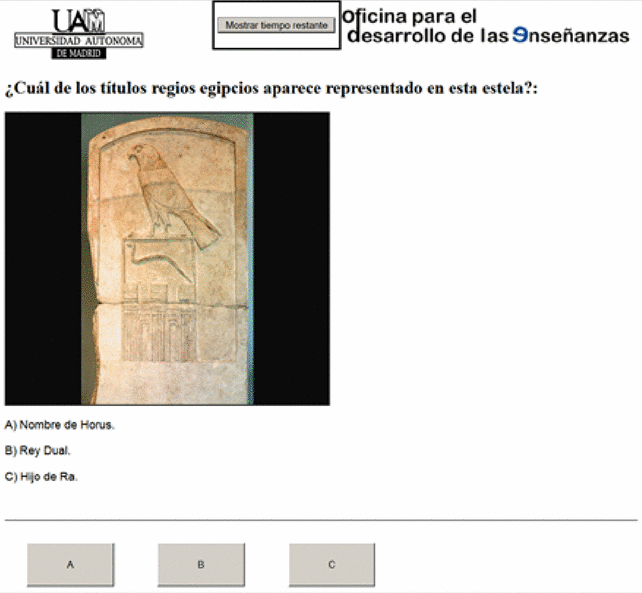
\includegraphics[width=0.75\textwidth,clip=true]{e-valUAM_primera_version}
	\caption{Interfaz del módulo del examen del primer prototipo}
	\label{fig:e-valUAM primera version}
\end{figure}

Desde el mes de octubre hasta el final del curso, los alumnos tuvieron disponibles 3 cuestionarios de auto evaluación y realizaron 4 exámenes. La auto evaluación estaba disponible a los alumnos tantas veces como quisieran. De los 15 alumnos, 6 utilizaron la aplicación para auto evaluación menos de 3 veces, mientras que otros 6 la utilizaron más de 15 veces. Los exámenes fueron dos parciales y un examen final para la convocatoria ordinaria y otra para la extraordinaria, al que solo se tuvieron que presentar 3 alumnos. La calificación determinada por la aplicación se ponderó en la nota final de la asignatura. A lo largo del año, entre tres profesores de Historia crearon un total de 372 preguntas, respondiéndose cada una de ellas 12,386 veces de media. 

Los resultados de la experiencia fueron muy satisfactorios. A nivel técnico, el sistema respondió como se esperaba durante todo el proceso, sin sufrir ningún tipo de caída. La mayor prueba de estrés del sistema fue el día del examen final. En las tres horas previas al examen se realizaron 31 accesos a los cuestionarios de auto evaluación, lo que supuso aproximadamente unas 300 peticiones al servidor. Cuando empezó el examen, los 15 alumnos lo realizaron a la vez, lo que supuso aproximadamente 68 peticiones por minuto al servidor durante los 20 minutos que duró el examen. El sistema logró almacenar todas las respuestas correctamente, seleccionar todas las preguntas siguientes siguiendo el modelo y ningún alumno tuvo que esperar entre preguntas ni sufrió ningún corte del servicio. Tampoco se registró ningún problema en los 3 meses que los alumnos hicieron un uso más intensivo del mismo (de noviembre de 2013 a enero de 2014).

% Hablar de qué se decidió cambiar
La experiencia de los alumnos con el sistema fue en general satisfactoria, aunque algunos mostraron malestar con el modelo del examen. Las mayores molestias venían provocadas porque no se pudieran dejar preguntas en blanco ni que se pudiera revisar una respuesta anterior. Aunque la segunda es una imposición del modelo (al depender las nuevas preguntas de las respuestas anteriores, estas no pueden cambiar), la primera sí se tuvo en consideración añadiendo la opción al modelo de la respuesta con duda.

De cara a la creación del segundo prototipo, además de añadir la respuesta con duda, se decidió crear el apartado de gestión del profesor, además de aumentar las capacidades de la aplicación para trabajar con ficheros multimedia. Así mismo, se hizo una actualización de la interfaz para incorporar un diseño responsive y adaptadarlo a toda las nuevas posibilidades multimedia que iban a incorporarse.

\section{2014/2015: Segundo prototipo}

Durante el curso académico 2014/2015 se utilizó en la asignatura de ``El Entorno como Instrumento Educativo'' del Grado en Educación Infantil. Las pruebas realizadas en este entorno fueron mucho más meticulosas que en el curso anterior, por varios motivos. 

Primero, los alumnos eran más y por lo tanto la aplicación se enfrentó a mayores picos de demanda. Segundo, se añadió más funcionalidad tanto para los profesores como para los alumnos. Tercero, los docentes utilizaron la aplicación como asistencia en su labor, pero además utilizamos la aplicación para conocer el nivel de conocimientos informáticos del que disponían los alumnos y conocer así mejor a los usuarios que iban a probar el sistema.



% Contar aquí que cambiamos el modelo

\subsection{Test de conocimientos informáticos}

\subsection{Alumnos del Grado en Educación Infantil}

\subsubsection{Aprendizaje}
\subsubsection{Examen final}
\subsubsection{Trabajo final}

\section{Comparativa con otras soluciones}